\chapter{Algorytmy samostrojenia}
\label{cha:ch8_algorytmy_samostrojenia}

W literaturze do teorii sterowania znajdują się opisy wielu klasycznych metod strojenia regulatorów, takich jak metoda Zieglera-Nicholsa \cite{KOWAL}\cite{CTRLENG} czy Åströma-Hägglunda \cite{CTRLENG}\cite{ASTROMHAGGLUND}. Wielu producentów oprogramowania serwonapędów lub sterowników technologicznych dostarcza własne algorytmy strojenia \textit{online} \cite{S7MANUAL}\cite{SCL_S71200_S71500}.

Zdecydowano się zrezygnować z metod klasycznych strojenia algorytmów, gdyż są one powszechnie znane i polegają na doprowadzeniu obiektu do cyklu granicznego, co w przypadku zastosowanej konstrukcji przeniesienia napędu można uzyskać podając stałe sterowanie na silnik. Prawdopodobnie dokładnie z takiego powodu oprogramowanie służące do programowania sterownika PLC --- \textsc{Siemens TIA Portal} --- nie było w stanie zakończyć poprawnie procesu samostrojenia regulatora pozycji belki.

Biorąc pod uwagę powyższe ograniczenia, zdecydowano się oprzeć samostrojenie regulatorów podrzędnego i nadrzędnego o automatyczne procesy identyfikacji matematycznych obiektów belki oraz kulki, co zostało opisane w niniejszym rozdziale.

%%%%
\section{Identyfikacja obiektu belki}
\label{sec:ch8_identyfikacja_belki}

Identyfikację belki oparto o odpowiedź skokową modelu obiektu pierwszego rzędu opisanego transmitancją:
\begin{equation}
    G_b(s) = \frac{K_b}{T_b s+1}
    \label{eq:transmitancja_obiektu_pierwszego_rzedu}
\end{equation}
gdzie $K_b$ oznacza wzmocnienie obiektu, a $T_b$ jego stałą czasową (\cite{KOWAL}). Parametry te można odczytać z~wykresu odpowiedzi skokowej (\cref{fig:odpowiedz_skokowa_obiektu_pierwszego_rzedu}, równanie \eqref{eq:odpowiedz_skokowa}) obiektu w następujący sposób:
\begin{itemize}
    \item wzmocnienie $K_b$ to iloraz wartości ustalonej $h_{ss}$ oraz zadanej amplitudy $A_\text{ref}$,
    \item stała czasowa $T_b$ równa jest ilorazowi pola powierzchni $S^+$ pod asymptotą i nad wykresem charakterystyki oraz wartości ustalonej.
\end{itemize}

\begin{equation}
    h(t) = h_{ss} \left( 1 - e^{-\frac{t}{T_b}} \right) \label{eq:odpowiedz_skokowa}
\end{equation}

Pole powierzchni $S^+$ (zobrazowane na \cref{fig:odpowiedz_skokowa_obiektu_pierwszego_rzedu}) określa się jako całkę:
\begin{nalign}
    S^+ &= \int \limits_{0}^{\infty} \left(h_{ss} - h(t) \right) \mathrm{d}x \\
        &= \int \limits_{0}^{\infty} \left(K_b A_\text{ref} - K_b A_\text{ref} + K_b A_\text{ref} e^{-\frac{t}{T_b}} \right) \mathrm{d}x \\
        &= T_b K_b A_\text{ref} e^{-\frac{t}{T_b}}|_{t=0}^{\infty} \\
        &= T_b K_b A_\text{ref} \label{eq:pole_nad_figura}
\end{nalign}

Przykładową odpowiedź skokową wału motoreduktora wraz z jej aproksymacją zaprezentowano na \cref{fig:identyfikacja_belki}. W celu identyfikacji zdecydowano się wykorzystać odczyt prędkości wału motoreduktora z~dwóch powodów:
\begin{itemize}
    \item po pierwsze, tylko prędkość kątowa wału jest wartością zachowującą się ściśle jak obiekt inercyjny pierwszego rzędu,
    \item po drugie, obrót belki zależny jest sinusoidalnie od obrotu wału silnika; stąd trudniejsze byłoby odczytanie parametrów ,,ukrytych'' w przebiegu sinusoidalnym, gdyby identyfikację przeprowadzano na kącie lub prędkości kątowej belki.
\end{itemize}
Algorytm identyfikacyjny (zob. rozdział \ref{sec:ch8_algorytm_identyfikacji_belki}) również korzysta z odpowiedzi skokowej wału motoreduktora.

\begin{figure}[ht]
    \centering
    \begin{tikzpicture}
        \begin{axis}[
            domain=0.0:3,
            xmin=0, xmax=2,
            ymin=0, ymax=40,
            samples=400,
            axis y line=center,
            axis x line=middle,
            legend pos=north west,
        ]
            \addplot+[name path=A, no marks] {25*(1-e^(-x/0.118))};
            \addlegendentry{Odpowiedź skokowa $h(t)$};
            \addplot[dashed,name path=B] {25};
            \addlegendentry{Wartość graniczna (stan ustalony) $h_{ss}$};
            \addplot[pattern=north east lines,pattern color=gray] fill between[of=A and B];
            \addlegendentry{Pole nad odpowiedzią skokową $S^+$};
        \end{axis}
    \end{tikzpicture}
    \caption{Wykres odpowiedzi skokowej obiektu inercyjnego pierwszego rzędu.}
    \label{fig:odpowiedz_skokowa_obiektu_pierwszego_rzedu}
\end{figure}

\begin{figure}[ht]
    \centering
    \includesvg[width=1\textwidth,svgpath=./vector_graphics/]{identyfikacja_belki}    
    \caption{Przykład aproksymacji odpowiedzi skokowej prędkości obrotowej wału motoreduktora.}
    \label{fig:identyfikacja_belki}
\end{figure}

Należy zwrócić uwagę, że wartością, która częściej jest wykorzystywana w algorytmach sterowania w tym obiekcie, jest nie prędkość kątowa wału motoreduktora, ale jego pozycja kątowa. Rozważany w procesie identyfikacji obiekt \eqref{eq:transmitancja_obiektu_pierwszego_rzedu} nie reprezentuje odpowiedzi kątowej silnika, dlatego należy użyć dodatkowego integratora, co pozwoli uzyskać kąt obrotu:
\begin{equation}
    H_b(s) = G_b(s) \cdot \frac{1}{s} = \frac{K_b}{T_b s^2 + s} \label{eq:transmitancja_silnik_odp_katowa}
\end{equation}

Obiektowi w ten sposób opisanemu odpowiadają następujące macierze stanu\footnote{Dzięki użyciu charakterystyki obiektu całkującego rzeczywistego \eqref{eq:transmitancja_silnik_odp_katowa} możliwe jest rozszerzenie macierzy wyjścia tak, aby móc odczytać dwa stany jednocześnie; nie jest to jednak wymagane w dalszej analizie, dlatego zostało pominięte.}:
\begin{nalign}
    A_I &= \begin{bmatrix}
        0 & 1 \\ 0 & -\frac{1}{T_b}
    \end{bmatrix} \\
    B_I &= \begin{bmatrix}
        0 \\ \frac{K_b}{T_b}
    \end{bmatrix} \\
    C_I &= \begin{bmatrix}
        1 & 0
    \end{bmatrix} \\
    D_I &= 0  \label{eq:macierze_stanu_obiektu_pierwszego_rzedu}
\end{nalign}

Regulator, który steruje belką, oparty jest o stan (kąt i prędkość kątową obrotu) belki (zob. rozdział \ref{sec:ch6_regulator_belki}), a jego nastawy obliczono wykorzystując funkcję \texttt{looptune} z programu \textsc{Matlab}, która optymalizuje zadany układ w dziedzinie częstotliwości. Przy samostrojeniu tego regulatora zdecydowano się na inne podejście oparte o przesuwanie wartości własnych zamkniętego układu. W tym celu wyliczono zależność algebraiczną pomiędzy nastawami regulatora a zadanymi wartościami własnymi.

Zamknięty układ regulacji z regulatorem od stanu $K_I = \begin{bmatrix}
    k_1 & k_2
\end{bmatrix}$ opisany jest równaniem:
\begin{equation}
    x' = \underbrace{(A_I - B_I K_I)}_{M \in \mathbb{C}^{2 \times 2}} x
\end{equation}

Macierz $M$ ma dwie wartości własne $\lambda_1$ oraz $\lambda_2$, które spełniają następujące zależności:
\begin{nalign}
    \det(M) &= \lambda_1 \lambda_2 \\
    \tr(M) &= \lambda_1 + \lambda_2 \label{eq:obiekt1_zaleznosc_lambd}
\end{nalign}

Dzięki \eqref{eq:obiekt1_zaleznosc_lambd} możliwe jest uzyskanie układu równań, po którego rozwiązaniu uzyskuje się następującą zależność na $K_I$:

\begin{nalign}
    k_1 &= \frac{\lambda_1 \lambda_2}{\frac{K_b}{T_b}} \\
    k_2 &= \frac{\frac{-1}{T_b} - \lambda_1 - \lambda_2}{\frac{K_b}{T_b}} \label{eq:zaleznosc_regulator_belki}
\end{nalign}

Należy zwrócić uwagę, że postać równań stanu obiektu \eqref{eq:macierze_stanu_obiektu_pierwszego_rzedu} nie do końca odpowiada postaci otrzymanej z linearyzacji \eqref{eq:rownania_stanu_belki} i \eqref{eq:rownania_wyjscia_belki}, w związku z tym zdecydowano się narzucić inne wartości własne macierzy $M$ niż te, które ma ,,zwinięty'' układ regulatora pozycji belki (\cref{fig:schemat_regulacji_belka}):

\begin{equation}
    \Lambda(M) = \begin{bmatrix}
    -8.2378 \\ -37.7286
    \end{bmatrix}
\end{equation}

%%%%
\section{Algorytm identyfikacji obiektu belki}
\label{sec:ch8_algorytm_identyfikacji_belki}

Opisany w rozdziale \ref{sec:ch8_identyfikacja_belki} eksperyment (odpowiedź skokowa prędkości kątowej wału motoreduktora) został zaimplementowany w sterowniku PLC, a jego wyniki służą do obliczania nowych nastaw regulatora według równań \eqref{eq:zaleznosc_regulator_belki}. Eksperyment polega na ustawieniu sterowania silnika na \SI{50}{\percent} na czas \SI{2}{\second}~i~zarejestrowaniu odczytu prędkości kątowej wału motoreduktora (jego odpowiedzi skokowej).

Procedura identyfikacyjna została przeprowadzona w sekwencji opisanej na \cref{fig:schemat_samostrojenia_belka}, a sama sekwencja została zaimplementowana w języku drabinkowym \textit{LAD} podobnie jak sekwencja bazowania czy sekwencja główna (rozdział \ref{sec:sekwencja_glowna}).

\begin{figure}[ht]
    \centering
    
    \begin{tikzpicture}[auto, node distance=1cm,>=latex']
    \node [startblock] (S1) {Reset zapisanych wartości};
    \node [block, below=2of S1] (S2) {Obliczanie całki pod wykresem};
    \node [block, right=of S2] (S3) {Zbieranie danych do obliczenia $h_{ss}$};
    \node [block, below=2of S2] (S4) {Obliczanie parametrów};
    \node [block, below=of S4] (S5) {Obliczanie regulatora};
        
    \draw [->] (S1) -- node [name=J1,left] {} node[name=T1,pos=0.75] {$T_1$} (S2);
    \draw [->] (J1) -| node [name=T2,pos=0.75] {$T_2$} (S3.north);
    \draw [->] (S2) -- node [name=J2,left] {} node[name=T3,pos=0.75] {$T_3$} (S4);
    \draw [-] (S3) |- (J2);
    \draw [->] (S4) -- (S5);
    \end{tikzpicture}
    
    \caption{Schemat sekwencji samostrojenia regulatora belki.}
    \label{fig:schemat_samostrojenia_belka}
\end{figure}

Tranzycjom $T_i$ zaznaczonym na schemacie na \cref{fig:schemat_samostrojenia_belka} odpowiadają następujące warunki:
\begin{itemize}
    \item $T_1$ -- rozpoczęcie eksperymentu (podanie sterowania \SI{50}{\percent} na silnik),
    \item $T_2$ -- upłynięcie czasu połowy eksperymentu (\SI{1}{\second}),
    \item $T_3$ -- zakończenie eksperymentu.
\end{itemize}

Krok pierwszy algorytmu, oznaczony jako \textit{Reset zapisanych wartości}, zeruje zapisaną wartość całki oraz dwa rejestry przechowujące sumę oraz ilość wartości, co uaktualniane jest co cykl procesora w~bloku \textit{Zbieranie danych do obliczenia $h_{ss}$}. Wartości te służą do obliczenia średniej arytmetycznej, która odpowiada oczekiwanej wartości ustalonej prędkości $h_{ss}$. Jest to wymuszone mocną kwantyzacją chwilowych wartości prędkości, co można zaobserwować na \cref{fig:identyfikacja_belki}.

Obliczanie całki odbywa się za pomocą bloku \texttt{LGF\_Integration}\cite{LGF} dostępnego w bibliotece \texttt{LGF} udostępnionej przez firmę \textsc{Siemens}. Na podstawie wzorów umieszczonych w rozdziale \ref{sec:ch8_identyfikacja_belki} obliczane są parametry $S$ (pole całkowite), $A_b$, $K_b$, $S^+$, $T_b$ oraz nastawy regulatora $k_1$, $k_2$.

%%%%
\section{Identyfikacja obiektu kulki}
\label{sec:ch8_identyfikacja_kulki}

Wykorzystując schemat sił działających na kulkę znajdującą się na pochylonej pod kątem $\theta$ belce (\cref{fig:sily_dzialajace_na_kulke}) wyznaczono, w sposób opisany poniżej, zależność przyspieszenia liniowego, które działa na kulkę, od kąta pochylenia belki.

\def\iangle{6} % Angle of the inclined plane
\def\arcr{1.1cm} % Radius of the arc used to indicate angles
\def\down{-90}

\begin{figure}[ht]
    \centering
    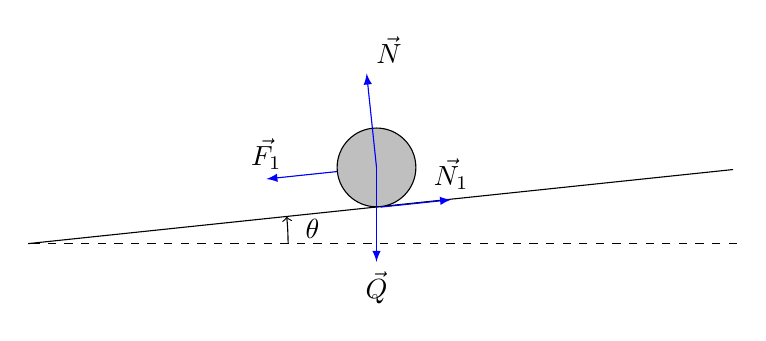
\begin{tikzpicture}[
        scale = 3,
        force/.style={>=latex,draw=blue,fill=blue},
        plane/.style={draw=black},
        M/.style={draw,circle,fill=lightgray,minimum size=1cm,thin},
        axis/.style={densely dashed,gray,font=\small},
    ]
        %\draw[plane] (0,-) coordinate (base) 
        %-- coordinate[pos=0.5] (mid) ++(\iangle:3) coordinate (top)
        %|- (base) -- cycle;
        \draw[dashed] (3,-1) -- (0,-1) coordinate (base);
        \draw (base)
        -- coordinate[pos=0.5] (mid) ++(\iangle:3) coordinate (top);
        \path (mid) node[M,rotate=\iangle,yshift=0.5cm] (M) {};
        \draw[->] (base)++(\arcr,0) arc (0:\iangle:\arcr);
        \path (base)++(\iangle*0.5:\arcr+3pt) node {$\theta$};
        
        \begin{scope}[rotate=\iangle]
            \draw [force,->] (M.center) -- ++(0,0.4) node[above right] {$\vec{N}$};
            % Assuming that Mg = 1. The normal force will therefore be cos(alpha)
            \draw [force,->] (M.west) -- ++(-0.3,0) node[above] {$\vec{F_1}$};
            \draw [force,->] (M.south) -- ++(0.3,0) node[above] {$\vec{N_1}$};
        \end{scope}
        \draw[force,->] (M.center) -- ++(0,-0.4) node[below] {$\vec{Q}$};
    \end{tikzpicture}
    
    \caption{Schemat sił działających na kulkę znajdującą się na pochylonej pod kątem $\theta$ belce.}
    \label{fig:sily_dzialajace_na_kulke}
\end{figure}

Zgodnie z rysunkiem, na kulkę działają dwie siły: $\vec{Q}$ (siła ciężkości) i $\vec{N}$ (siła reakcji podłoża). Dodatkowo zostały zaznaczone składowe równoległe do powierzchni belki wspomnianych sił, $\vec{F_1}$ oraz $\vec{N_1}$; ich wypadkowa $F = am = F_1 - N_1$ jest siłą powodującą staczanie się kulki z przyspieszeniem wypadkowym $a$ wzdłuż belki.

Wartość siły ciężkości działającej na kulkę definiowana jest jako $Q=mg$, gdzie $m$ to masa kulki, a~$g$~to przyspieszenie ziemskie. Automatycznie składowa $F_1$ ma wartość $F_1=mg\sin\theta$.

Siła $\vec{N_1}$, pochodząca od tarcia suchego kulki o belkę, wprowadza kulkę w ruch obrotowy, stąd $\epsilon J = r N_1$, gdzie $\epsilon$ to przyspieszenie kątowe kulki, $J$ to moment bezwładności kulki, a $r$ to jej promień. Dodatkowo pojawia się zależność przyspieszenia liniowego od kątowego $a = \epsilon r$, która jest właściwa przy braku poślizgu kulki o belkę.

Podstawiając wartości sił $F_1$ i $N_1$ do równania na siłę wypadkową działającą na kulkę otrzymano:

\begin{nalign}
    F &= mg\sin\theta - \frac{\epsilon}{r}J \\
    a m &= mg\sin\theta - \frac{a}{r^2}J \\
    a\left(m + \frac{J}{r^2} \right) &= mg\sin\theta \\
    a &= \frac{mg\sin\theta}{m+\frac{J}{r^2}} \\
      &= \frac{r^2mg\sin\theta}{r^2m+J}
    \label{eq:przyspieszenie_kulki1}
\end{nalign}

Wiadomo, że moment bezwładności $J$ jednolitej kulki o promieniu $r$ wynosi $J=\frac{2}{5}r^2m$. Podstawiając ten wzór do wyniku z \eqref{eq:przyspieszenie_kulki1} otrzymano:

\begin{nalign}
    a &= \frac{r^2mg\sin\theta}{r^2m+J}\\
      &= \frac{r^2mg\sin\theta}{r^2m+\frac{2}{5}r^2m} \\
      &= \frac{g\sin\theta}{1+\frac{2}{5}} \\
      &= \frac{5}{7} g \sin\theta
    \label{eq:przyspieszenie_kulki2}
\end{nalign}

Wartość $\frac{5}{7}g$ to w przybliżeniu 7, natomiast dla małych kątów $\sin\theta \approx \theta$. Stąd ostateczny wynik:

\begin{equation}
    a \approx 7 \cdot \theta \label{eq:przyspieszenie_kulki3}
\end{equation}

Oznacza to, że przyspieszenie kulki staczającej się po pochylonej belce jest stałe i wynosi około siedmiokrotność kąta pochylenia belki. Należy w tym miejscu zwrócić uwagę na wyniki linearyzacji \eqref{eq:rownania_stanu_kulki2} oraz \eqref{eq:rownania_wyjscia_kulki2}, które zostały przypomniane poniżej:

\begin{align*}
    \begin{bmatrix}
        \dot{x}_1 \\ \dot{x}_2
    \end{bmatrix}
    &= \begin{bmatrix}
        0 & 1 \\
        0 & 0
    \end{bmatrix}
    \begin{bmatrix}
        x_1 \\ x_2
    \end{bmatrix}
    +
    \begin{bmatrix}
        0 & 0 \\ 7,0047 & 0
    \end{bmatrix}
    \begin{bmatrix}
        u_1^* \\ u_2^*
    \end{bmatrix}\\
    \begin{bmatrix}
        y_1 \\ y_2
    \end{bmatrix}
    &= \begin{bmatrix}
        1 & 0 \\
        0 & 1 \\
    \end{bmatrix}
    \begin{bmatrix}
        x_1 \\ x_2
    \end{bmatrix}
    + \begin{bmatrix}
        -0,0675 & 0 \\
        0 & -0.0675
    \end{bmatrix}
    \begin{bmatrix}
        u_1^* \\ u_2^*
    \end{bmatrix}
\end{align*}

Jak widać po równaniach stanu, $x_1$ jest całką $x_2$, a pochodna stanu $x_2$ --- $\dot{x}_2$ --- jest siedmiokrotnością sterowania $u_1^*$. Wyniki te są zgodne z otrzymaną zależnością \eqref{eq:przyspieszenie_kulki3}, gdyż $x_1$ to pozycja liniowa kulki, $x_2$ to jej prędkość liniowa, $\dot{x}_2$ to przyspieszenie liniowe, a $u_1^*$ to kąt belki.

Powyższy wywód dowodzi, że przyspieszenie kulki, które charakteryzuje jej dynamikę, jest niezależne od momentu bezwładności kulki --- czyli od jej masy i rozmiaru --- a~zatem eksperymenty identyfikacyjne (takie jak pomiar czasu i/lub drogi staczania się kulki) nie dadzą rezultatów, które mogłyby w jakikolwiek sposób pomóc w doborze regulatora.

Regulator nadrzędny został zbudowany dla systemu ,,zwiniętego'' (zob. rozdział \ref{sec:ch6_regulator_kulki}), obejmującego wewnętrzną pętlę sprzężenia zwrotnego dla systemu belki oraz system kulki, a zatem po zmianie parametrów tej pętli wewnętrznej można ponownie przeprowadzić obliczenia dające nowe nastawy regulatora nadrzędnego. Po przeprowadzeniu takich obliczeń z wykorzystaniem funkcji \texttt{looptune} okazało się, że ,,nowe'' nastawy są zbliżone do nastaw regulatora dla modelu zlinearyzowanego, dlatego zdecydowano się pominąć te obliczenia w procesie samostrojenia.

%%%%
\section{Podsumowanie}

W niniejszym rozdziale zaprezentowano metodę samostrojenia regulatora podrzędnego opartą o identyfikację modelu matematycznego obiektu inercyjnego pierwszego rzędu, jakim jest silnik użyty w obiekcie regulacji. Opisano również matematyczne zależności między parametrami takiego modelu a jego odpowiedzią skokową. Następnie przeprowadzono obliczenia zależności pomiędzy regulatorem od stanu, obiektem inercyjnym pierwszego rzędu oraz zadanymi wartościami własnymi układu z zamkniętą pętlą sprzężenia zwrotnego. W kolejnej części rozdziału opisano implementację procedury samostrojenia, wykorzystującą zależności parametrów obiektu i odpowiedzi skokowej, na sterowniku PLC.

Na koniec przeprowadzono wywód udowadniający, że przeprowadzona identyfikacja kulki nie powiedzie się, gdyż jej model liniowy jest niezależny od parametrów fizycznych kulki, a jedynie od kąta obrotu belki. Z tego powodu zaniechano implementacji procedury samostrojenia dla kulki.

%---------------------------------------------------------------------------